\documentclass[11pt,letterpaper]{article}
\input{glyphtounicode}
\pdfgentounicode=1
\usepackage[utf8]{inputenc}
\usepackage[T1]{fontenc}
\usepackage{lmodern}
\usepackage[spanish,es-noindentfirst,es-tabla]{babel}
\decimalpoint
\usepackage[margin=2.5cm]{geometry}
\usepackage{graphicx}
\usepackage{booktabs}
\usepackage{array}
\usepackage{multirow}
\usepackage{siunitx}
\sisetup{output-decimal-marker={.}, group-digits=false, detect-weight=true, table-number-alignment=center}
\usepackage{amsmath,amssymb}
\usepackage{listings}
\renewcommand{\lstlistingname}{Código}
\usepackage{xcolor}
\usepackage{tikz}
\usetikzlibrary{positioning,arrows.meta,shapes.geometric}
\usepackage{fancyhdr}
\usepackage{titlesec}
\usepackage{caption}
\usepackage[section]{placeins}
\usepackage[hidelinks]{hyperref}
\graphicspath{{figuras/}}
\renewcommand{\topfraction}{0.92}
\renewcommand{\bottomfraction}{0.85}
\renewcommand{\textfraction}{0.06}
\renewcommand{\floatpagefraction}{0.80}
\setcounter{topnumber}{3}
\setcounter{totalnumber}{5}
\captionsetup{font=small,labelfont=bf}

\lstdefinestyle{codigo}{
    language=Python,
    basicstyle=\ttfamily\footnotesize,
    keywordstyle=\color{blue!60!black}\bfseries,
    commentstyle=\color{gray},
    stringstyle=\color{orange!70!black},
    numbers=left,
    numberstyle=\tiny\color{gray},
    frame=single,
    breaklines=true,
    showstringspaces=false,
    tabsize=4,
    backgroundcolor=\color{gray!5},
    extendedchars=true,
    columns=fullflexible,
    keepspaces=true,
    literate={á}{{\'a}}1 {é}{{\'e}}1 {í}{{\'i}}1 {ó}{{\'o}}1 {ú}{{\'u}}1
             {Á}{{\'A}}1 {É}{{\'E}}1 {Í}{{\'I}}1 {Ó}{{\'O}}1 {Ú}{{\'U}}1
             {ñ}{{\~n}}1 {Ñ}{{\~N}}1 {¿}{{?`}}1 {¡}{{!`}}1 {±}{{$\pm$}}1
}
\lstset{style=codigo}

\pagestyle{fancy}
\fancyhf{}
\rhead{Inteligencia Computacional Aplicada}
\cfoot{\thepage}
\renewcommand{\headrulewidth}{0.4pt}
\titleformat{\section}{\normalfont\Large\bfseries}{\thesection.}{0.5em}{}
\titleformat{\subsection}{\normalfont\large\bfseries}{\thesubsection}{0.5em}{}

\newcommand{\nombreEstudiante}{Sergio Santiago Duarte Rojas}
\newcommand{\codigoEstudiante}{20261595002}
\newcommand{\nombreDocente}{Cesar Andrey Perdomo Charry}
\newcommand{\nombreAsignatura}{Inteligencia Computacional Aplicada}

% Diagramas de arquitectura
\definecolor{cEntrada}{RGB}{230,230,230}
\definecolor{cConv}{RGB}{204,224,240}
\definecolor{cPool}{RGB}{255,228,204}
\definecolor{cDensa}{RGB}{212,236,222}
\definecolor{cReg}{RGB}{236,220,240}
\tikzset{
    capa/.style={draw=black!60, rounded corners=2pt, minimum height=1.05cm, text width=1.95cm, align=center, font=\footnotesize, inner sep=2pt},
    tensor/.style={font=\scriptsize, text=black!70},
    flecha/.style={-{Latex[length=1.6mm]}, black!70},
}

\input{cifras}
\hypersetup{pdftitle={Actividad 3. Taller resuelto de aprendizaje profundo}, pdfauthor={Sergio Santiago Duarte Rojas}}
\lhead{Actividad 3, taller resuelto}

\begin{document}

\begin{titlepage}
    \centering
    \vspace*{2cm}
    {\LARGE \bfseries Actividad 3. Taller resuelto\\[4pt] Reconocimiento de dígitos manuscritos con redes profundas\par}
    \vspace{0.5cm}
    {\large Informe de ejecución\par}
    \vspace{2cm}
    \begin{tabular}{ll}
        \textbf{Asignatura:} & \nombreAsignatura \\
        \textbf{Docente:}    & \nombreDocente \\
        \textbf{Estudiante:} & \nombreEstudiante \\
        \textbf{Código:}     & \codigoEstudiante \\
        \textbf{Fecha:}      & \today \\
    \end{tabular}
    \vfill
    Universidad Distrital Francisco José de Caldas
\end{titlepage}

\tableofcontents
\newpage

\section{Introducción}

El Taller 2 cerró con un perceptrón multicapa entrenado por retropropagación sobre vectores de pocas entradas. Este taller lleva la misma idea a imágenes. El cuaderno del docente entrena dos redes sobre MNIST (LeCun et al., 1998), 70\,000 dígitos manuscritos de $28\times28$ píxeles, primero un perceptrón multicapa que trata la imagen como un vector de 784 números y después una red convolucional que la trata como una imagen. El informe documenta la ejecución, confirma los puntos de control y explica lo que muestran las curvas, la matriz de confusión y el experimento con la tasa de aprendizaje.

El cuaderno se ejecutó completo y sin modificaciones, con PyTorch 2.12 (Paszke et al., 2019) sobre una GPU NVIDIA y semilla 42. MNIST se descargó con torchvision, sin recurrir al conjunto de respaldo que el cuaderno trae para cuando no hay conexión. Las diez verificaciones de los cinco puntos de control dieron \texttt{[OK]}.

\section{Marco teórico (resumen)}

\subsection{De vectores a imágenes}

El MLP del Taller 2 recibe un vector y lo pasa por capas densas, en las que cada neurona se conecta con todas las entradas. Aplicado a una imagen, eso obliga a aplanarla, con lo que se pierde la noción de vecindad entre píxeles y el número de pesos crece con el tamaño de la imagen. Una capa convolucional desliza un filtro pequeño, aquí de $3\times3$, por toda la imagen y calcula en cada posición una suma ponderada con los mismos pesos. Un filtro aprende entonces un rasgo local, un borde o un trazo, y lo detecta en cualquier posición. Una capa con $c_{in}$ canales de entrada, $c_{out}$ filtros y tamaño $k$ tiene $c_{out}(c_{in}k^2+1)$ parámetros, sin importar el tamaño de la imagen. Sin relleno (píxeles de valor cero añadidos alrededor de la imagen) la salida pierde $k-1$ píxeles por eje. La activación ReLU, $\max(0, z)$, es la misma del Taller 2. El \emph{max pooling} toma el máximo de cada ventana de $2\times2$ y reduce la imagen a la mitad por lado, lo que da cierta tolerancia a desplazamientos de un píxel y abarata las capas siguientes.

\subsection{Pérdida y optimizador}

Con diez clases la salida de la red son diez \emph{logits} $z_k$. La función softmax los convierte en probabilidades, $p_k = e^{z_k}/\sum_j e^{z_j}$, y la pérdida es la entropía cruzada $L = -\ln p_y$, donde $y$ es la clase correcta. Es la misma cadena de retropropagación del Taller 2 con otra activación de salida y otra medida de error. Para una red que reparte la probabilidad por igual entre las diez clases vale $\ln 10 = 2.303$, una referencia útil para leer las tablas. Adam (Kingma y Ba, 2015) combina el momento del Taller 2, un promedio móvil del gradiente, con un segundo promedio móvil del gradiente al cuadrado que normaliza el paso de cada peso, de modo que una misma tasa de aprendizaje sirve para pesos con gradientes de magnitudes muy distintas. El \emph{dropout} (Srivastava et al., 2014) apaga al azar una fracción $p$ de las activaciones en cada paso de entrenamiento y reescala las restantes por $1/(1-p)$, para que la evaluación, que usa todas, vea activaciones de la misma escala.

\section{Metodología}

\subsection{Datos y particiones}

MNIST trae 60\,000 imágenes de entrenamiento y 10\,000 de prueba. El cuaderno aparta \nVal{} imágenes del entrenamiento como validación, deja \nTr{} para entrenar y reserva la prueba para la evaluación final. Los píxeles se llevan de 0 a 255 al rango 0 a 1 y después se normalizan con la media (\media) y la desviación (\desv) calculadas solo sobre el entrenamiento. El desbalance entre clases es moderado, la más numerosa tiene un \conteoDifPct{} \% más imágenes que la menos numerosa. La Figura~\ref{fig:muestras} muestra las primeras dieciséis.

\begin{figure}[!htb]
    \centering
    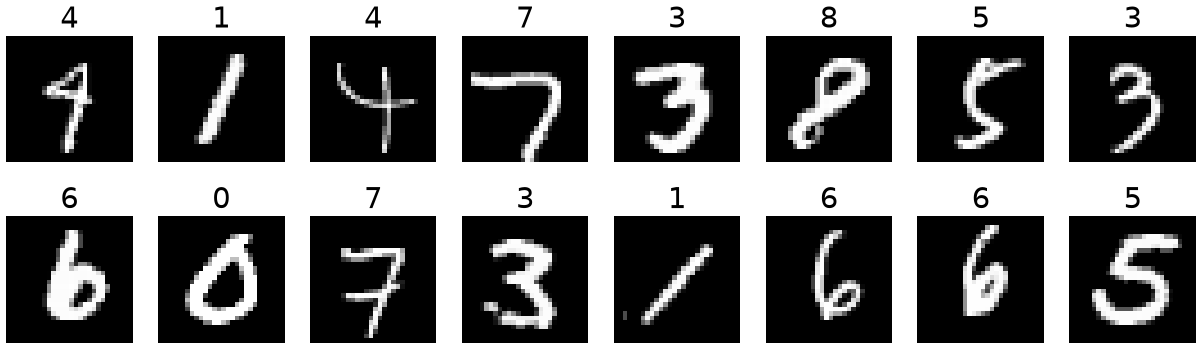
\includegraphics[width=13cm]{fig01_muestras.png}
    \caption{Primeras dieciséis imágenes de entrenamiento con su etiqueta}
    \label{fig:muestras}
\end{figure}

\subsection{Arquitecturas}

La Tabla~\ref{tab:arq} y la Figura~\ref{fig:arq} describen las dos redes. El MLP aplana la imagen y tiene una capa oculta de 128 neuronas con ReLU, \paramMlp{} parámetros. La CNN tiene dos bloques de convolución $3\times3$ seguida de ReLU y \emph{max pooling}, un \emph{dropout} de 0.25 y una capa lineal, \paramCnn{} parámetros, \razonParam{} veces menos que el MLP. Ambas devuelven diez \emph{logits} y la softmax va dentro de la pérdida.

\begin{table}[!htb]
    \centering
    \caption{Capas de las dos redes. En la CNN las convoluciones no usan relleno, así que cada una quita un píxel por lado}
    \label{tab:arq}
    \footnotesize
    \begin{tabular}{llr}
        \toprule
        \textbf{Red} & \textbf{Capa} & \textbf{Parámetros} \\
        \midrule
        \multirow{3}{*}{MLP} & Aplanar, 784 & 0 \\
                             & Lineal 784 a 128 con ReLU & 100\,480 \\
                             & Lineal 128 a 10 & 1\,290 \\
        \midrule
        \multirow{6}{*}{CNN} & Convolución $3\times3$, 16 filtros, ReLU, salida $16\times26\times26$ & 160 \\
                             & Max pooling $2\times2$, salida $16\times13\times13$ & 0 \\
                             & Convolución $3\times3$, 32 filtros, ReLU, salida $32\times11\times11$ & 4\,640 \\
                             & Max pooling $2\times2$, salida $32\times5\times5$ & 0 \\
                             & Aplanar, 800, y dropout 0.25 & 0 \\
                             & Lineal 800 a 10 & 8\,010 \\
        \bottomrule
    \end{tabular}
\end{table}

\begin{figure}[!htb]
    \centering
    \begin{tikzpicture}[node distance=0.35cm]
        \node[capa, fill=cEntrada] (e) {Entrada\\$1\times28\times28$};
        \node[capa, fill=cDensa, right=of e] (f) {Aplanar\\784};
        \node[capa, fill=cDensa, right=of f] (h) {Lineal 128\\ReLU};
        \node[capa, fill=cDensa, right=of h] (o) {Lineal 10\\logits};
        \draw[flecha] (e) -- (f); \draw[flecha] (f) -- (h); \draw[flecha] (h) -- (o);
        \node[tensor, above=0.1cm of f] {MLP, \paramMlp{} parámetros};
        %
        \node[capa, fill=cEntrada, below=1.1cm of e] (e2) {Entrada\\$1\times28\times28$};
        \node[capa, fill=cConv, right=of e2] (c1) {Conv $3\times3$\\16 filtros, ReLU};
        \node[capa, fill=cPool, right=of c1] (p1) {Max pooling\\$2\times2$};
        \node[capa, fill=cConv, right=of p1] (c2) {Conv $3\times3$\\32 filtros, ReLU};
        \node[capa, fill=cPool, right=of c2] (p2) {Max pooling\\$2\times2$};
        \node[capa, fill=cReg, below=0.45cm of p2] (dr) {Aplanar 800\\Dropout 0.25};
        \node[capa, fill=cDensa, left=of dr] (o2) {Lineal 10\\logits};
        \draw[flecha] (e2) -- (c1); \draw[flecha] (c1) -- (p1); \draw[flecha] (p1) -- (c2); \draw[flecha] (c2) -- (p2);
        \draw[flecha] (p2) -- (dr); \draw[flecha] (dr) -- (o2);
        \node[tensor, above=0.02cm of c1] {$16\times26\times26$};
        \node[tensor, above=0.02cm of p1] {$16\times13\times13$};
        \node[tensor, above=0.02cm of c2] {$32\times11\times11$};
        \node[tensor, above=0.02cm of p2] {$32\times5\times5$};
        \node[tensor, below=0.02cm of e2] {CNN, \paramCnn{} parámetros};
    \end{tikzpicture}
    \caption{Las dos redes del cuaderno. Encima de cada bloque de la CNN va el tamaño de su salida, canales por alto por ancho}
    \label{fig:arq}
\end{figure}

\subsection{Entrenamiento y evaluación}

Las dos redes se entrenan 3 épocas con Adam, tasa $10^{-3}$, lotes de 64 imágenes en orden aleatorio y entropía cruzada. Conviene tener presente cómo mide el cuaderno cada cifra. La pérdida y la exactitud de entrenamiento son el promedio de los lotes de la época, calculado mientras los pesos todavía cambian y con el \emph{dropout} activo. La pérdida y la exactitud de validación se miden al final de la época, con la red ya actualizada y en modo de evaluación. Las dos columnas no son comparables al detalle y eso explica parte de lo que se ve en las curvas. La prueba se evalúa una vez con la CNN entrenada y otra vez solo para comprobar el modelo recargado desde disco.

El cuaderno pide anotar una predicción antes del experimento con la tasa de aprendizaje, que repite el entrenamiento de la CNN durante 2 épocas con $10^{-1}$, $10^{-3}$ y $10^{-5}$. Lo esperado era que $10^{-1}$ fuera demasiado grande para Adam y la red no aprendiera, que $10^{-5}$ aprendiera pero quedara lejos en 2 épocas y que $10^{-3}$ repitiera el resultado principal.

\section{Resultados}

\subsection{Curvas de aprendizaje}

La Tabla~\ref{tab:epocas} y la Figura~\ref{fig:curvas} recogen las tres épocas de cada red. La CNN termina con \vaccCnnC{} \% de validación frente a \vaccMlpC{} del MLP, \difVal{} puntos más, y su pérdida de validación es la mitad. Las dos cifras quedan dentro de los rangos orientativos del cuaderno, 96 a 98 \% para el MLP y 98.5 a 99.2 para la CNN.

\begin{table}[!htb]
    \centering
    \caption{Pérdida y exactitud por época. La exactitud está en porcentaje. Las columnas de entrenamiento son promedios de la época y las de validación se miden al final de ella}
    \label{tab:epocas}
    \footnotesize
    \begin{tabular}{l c S[table-format=1.4] S[table-format=2.2] S[table-format=1.4] S[table-format=2.2]}
        \toprule
         & & \multicolumn{2}{c}{\textbf{Entrenamiento}} & \multicolumn{2}{c}{\textbf{Validación}} \\
        \cmidrule(lr){3-4} \cmidrule(lr){5-6}
        \textbf{Red} & \textbf{Época} & {\textbf{Pérdida}} & {\textbf{Exactitud}} & {\textbf{Pérdida}} & {\textbf{Exactitud}} \\
        \midrule
        \multirow{3}{*}{MLP} & 1 & \lossMlpA & \accMlpA & \vlossMlpA & \vaccMlpA \\
                             & 2 & \lossMlpB & \accMlpB & \vlossMlpB & \vaccMlpB \\
                             & 3 & \lossMlpC & \accMlpC & \vlossMlpC & \vaccMlpC \\
        \midrule
        \multirow{3}{*}{CNN} & 1 & \lossCnnA & \accCnnA & \vlossCnnA & \vaccCnnA \\
                             & 2 & \lossCnnB & \accCnnB & \vlossCnnB & \vaccCnnB \\
                             & 3 & \lossCnnC & \accCnnC & \vlossCnnC & \vaccCnnC \\
        \bottomrule
    \end{tabular}
\end{table}

\begin{figure}[!htb]
    \centering
    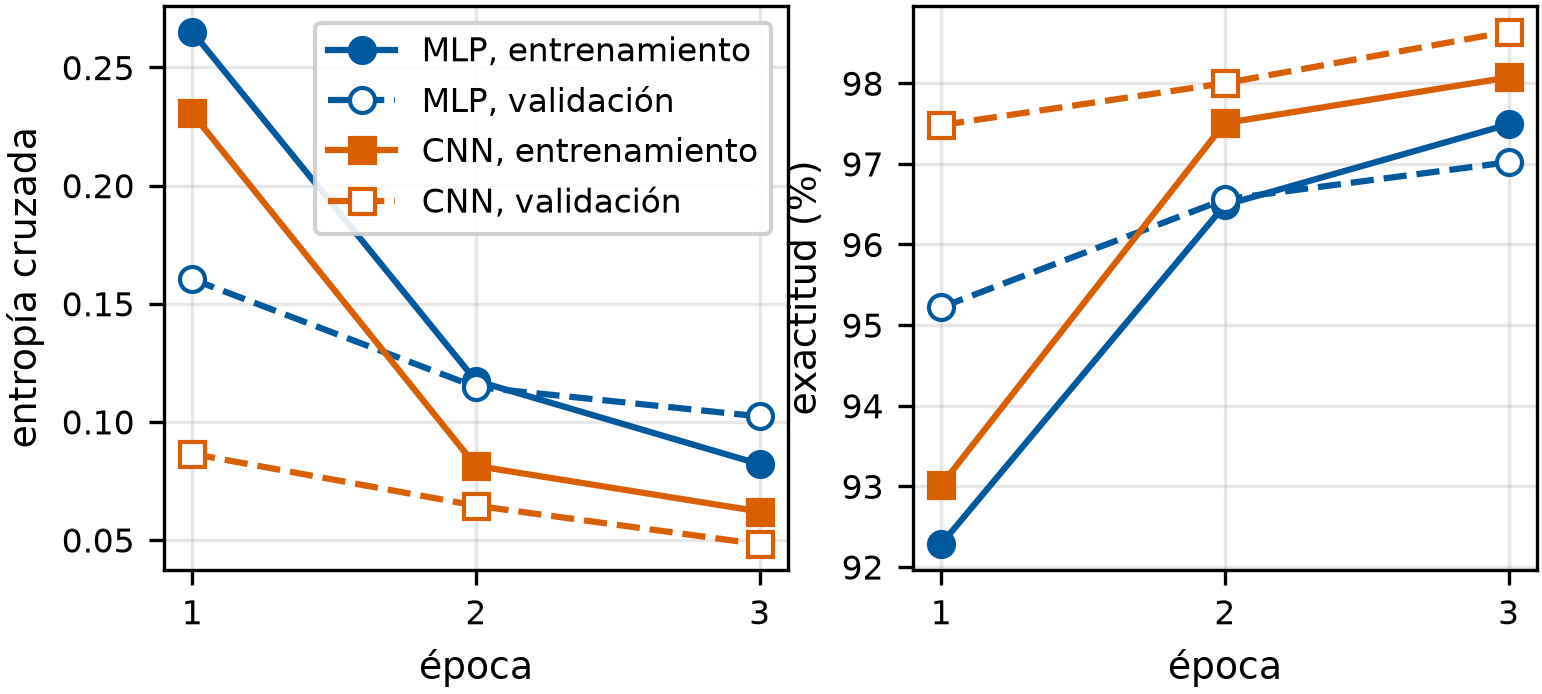
\includegraphics[width=15cm]{fig02_curvas.png}
    \caption{Pérdida y exactitud por época de las dos redes. Línea continua y marcador lleno para el entrenamiento, discontinua y marcador hueco para la validación}
    \label{fig:curvas}
\end{figure}

\subsection{Evaluación en prueba}

La CNN acierta \accTe{} \% de las \nTe{} imágenes de prueba, \erroresTe{} errores, con pérdida \perdTe. La Figura~\ref{fig:confusion} muestra la matriz de confusión y la Tabla~\ref{tab:clases} el acierto por clase, que va de \accPeor{} \% en el \clasePeor{} a \accMejor{} en el \claseMejor. Los errores se reparten por \celdasConError{} de las 90 celdas fuera de la diagonal. Los tres pares más frecuentes, \parAA{} tomado por \parAB{}, \parBA{} por \parBB{} y \parCA{} por \parCB, reúnen \tresParesN{} errores, el \tresParesPct{} \% del total. La columna del \colMaxDig{} recibe \colMaxN{} errores de otras clases y por eso ese dígito tiene la precisión más baja. La Figura~\ref{fig:errores} muestra los diez primeros errores.

\begin{figure}[!htb]
    \centering
    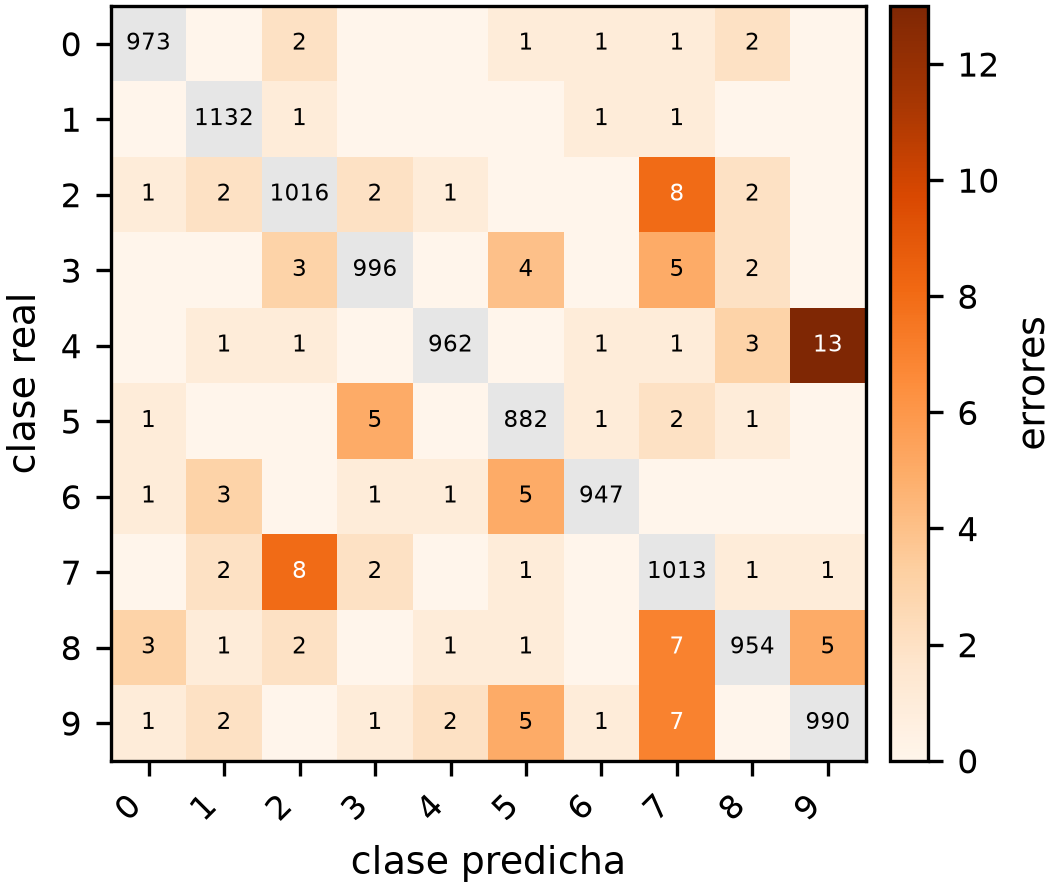
\includegraphics[width=9cm]{fig03_confusion.png}
    \caption{Matriz de confusión de la CNN sobre las \nTe{} imágenes de prueba. El color codifica solo los errores y la diagonal va en gris para que los aciertos no aplanen la escala}
    \label{fig:confusion}
\end{figure}

\begin{table}[!htb]
    \centering
    \caption{Acierto por clase en prueba. El acierto es la fracción de imágenes de la clase bien clasificadas y la precisión la fracción de predicciones de esa clase que eran correctas}
    \label{tab:clases}
    \footnotesize
    \begin{tabular}{l S[table-format=4.0] S[table-format=4.0] S[table-format=2.1] S[table-format=2.1]}
        \toprule
        \textbf{Dígito} & {\textbf{Imágenes}} & {\textbf{Aciertos}} & {\textbf{Acierto (\%)}} & {\textbf{Precisión (\%)}} \\
        \midrule
\filasPorClase
        \bottomrule
    \end{tabular}
\end{table}

\begin{figure}[!htb]
    \centering
    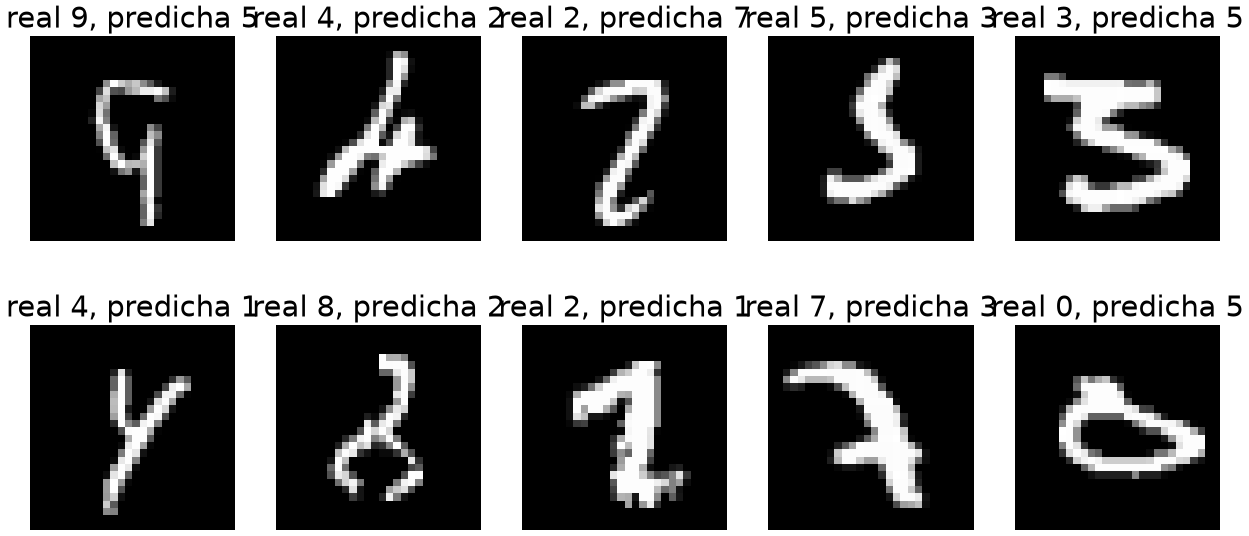
\includegraphics[width=13cm]{fig04_errores.png}
    \caption{Los diez primeros errores de la CNN en prueba, con la clase real y la predicha}
    \label{fig:errores}
\end{figure}

\subsection{Tasa de aprendizaje}

La Tabla~\ref{tab:lr} resume el experimento de 2 épocas y confirma la predicción. Con $10^{-1}$ la red queda en \lrAAcc{} \% y su pérdida de validación se queda a \lrAMilesimas{} milésimas de $\ln 10$. Con $10^{-5}$ llega a \lrCAcc{} \% con una pérdida todavía alta y con $10^{-3}$ alcanza \lrBAcc{} \%.

\begin{table}[!htb]
    \centering
    \caption{CNN tras 2 épocas con tres tasas de aprendizaje. La pérdida de entrenamiento es el promedio de cada época}
    \label{tab:lr}
    \footnotesize
    \begin{tabular}{S[table-format=1.0e-1] S[table-format=1.2] S[table-format=1.2] S[table-format=2.2] S[table-format=1.4]}
        \toprule
        {\textbf{Tasa}} & {\textbf{Pérdida ent. época 1}} & {\textbf{Pérdida ent. época 2}} & {\textbf{Exactitud val. (\%)}} & {\textbf{Pérdida val.}} \\
        \midrule
        1e-1 & \lrATrLossA & \lrATrLossB & \lrAAcc & \lrALoss \\
        1e-3 & \lrBTrLossA & \lrBTrLossB & \lrBAcc & \lrBLoss \\
        1e-5 & \lrCTrLossA & \lrCTrLossB & \lrCAcc & \lrCLoss \\
        \bottomrule
    \end{tabular}
\end{table}

\subsection{Modelo guardado}

Los pesos de la CNN se guardaron en disco, se cargaron en una red nueva y la exactitud de prueba fue la misma, así que el modelo se puede reutilizar sin entrenarlo otra vez.

\section{Análisis}

\subsection{Por qué gana la CNN con menos parámetros}

El MLP gasta 100\,480 de sus parámetros en conectar cada píxel con cada neurona oculta, y cada uno de esos pesos solo sirve para una posición de la imagen. La primera capa de la CNN tiene 160 parámetros porque sus 16 filtros se reutilizan en las 676 posiciones de la imagen, y el \emph{pooling} hace que un trazo movido un píxel active casi lo mismo. Con \razonParam{} veces menos parámetros la CNN mejora la validación en \difVal{} puntos y reduce la pérdida a la mitad. Esa es la explicación habitual, el cuaderno no incluye un experimento que la aísle, pero la diferencia de resultados es consistente con ella.

\subsection{Qué dicen las curvas}

En las dos redes la validación supera al entrenamiento en la primera época, \vaccMlpA{} frente a \accMlpA{} en el MLP y \vaccCnnA{} frente a \accCnnA{} en la CNN. El MLP no tiene \emph{dropout}, así que la causa principal no puede ser esa. Es la forma de medir descrita en la Sección 3.3. La exactitud de entrenamiento es un promedio de toda la época, que arranca con una red casi al azar, mientras que la validación se mide con la red que queda al final. A medida que la red cambia menos de una época a otra la diferencia se cierra, y en la tercera época el MLP ya supera a la validación por \brechaMlpC{} puntos. En la CNN la validación sigue por encima en las tres épocas porque el \emph{dropout} añade una segunda causa, entrena con el 75 \% de las 800 características y evalúa con todas.

El MLP no muestra sobreajuste en tres épocas. Su pérdida de validación sigue bajando y la diferencia de \brechaMlpC{} puntos en la última época es una brecha de generalización pequeña, no una divergencia entre las curvas como la que el Taller 2 mostró en Breast Cancer. Con más épocas sería el primer sitio donde mirar.

\subsection{Qué dígitos se confunden}

Los errores no se concentran en unos pocos pares. Ocupan \celdasConError{} de las 90 celdas fuera de la diagonal y los tres pares más frecuentes solo reúnen el \tresParesPct{} \% de ellos. Lo que sí se ve es una estructura. Los pares \parAA{} con \parAB{} y \parBA{} con \parBB{} son dígitos que difieren en un trazo, un 4 con la parte superior cerrada se convierte en un 9 y un 7 con el trazo horizontal curvo se parece a un 2. La columna del \colMaxDig{} recibe más errores que ninguna otra, \colMaxN{}, lo que sugiere que la forma del 7, un trazo horizontal y otro inclinado, aparece como fragmento en dígitos de otras clases mal escritos. De los diez errores de la Figura~\ref{fig:errores} solo uno pertenece a los tres pares principales y varios son dígitos que una persona también dudaría en clasificar.

\subsection{Qué muestra la tasa de aprendizaje}

Con $10^{-1}$ la pérdida de entrenamiento de la primera época, \lrATrLossA, supera a $\ln 10$. Adam da pasos de tamaño cercano a la tasa sin importar la magnitud del gradiente, así que los pesos saltan a valores que ya no dependen de la imagen y la red colapsa a una salida casi constante. Una exactitud de \lrAAcc{} \% corresponde a predecir casi siempre la misma clase, y una pérdida a \lrAMilesimas{} milésimas de $\ln 10$ dice que la salida constante reparte la probabilidad casi por igual entre las diez clases. Con $10^{-5}$ la pérdida sí baja época a época, así que la red aprende, pero necesitaría muchas más épocas. El valor intermedio de $10^{-3}$ repite la lección del Taller 2 con la tasa del MLP, demasiado grande no aprende y demasiado pequeña no llega a tiempo.

La ejecución con $10^{-3}$ de este experimento no repite las cifras de la Tabla~\ref{tab:epocas} en sus dos primeras épocas. La función que fija la semilla reinicia los generadores de PyTorch pero no el generador propio que el cuaderno le entrega al cargador de datos, así que el orden de los lotes cambia de una ejecución a otra. Además algunas operaciones de la convolución en GPU no son deterministas, y por eso la CNN cambia en la segunda cifra decimal entre ejecuciones completas del cuaderno mientras que el MLP repite sus cifras.

\section{Conclusiones}

La red convolucional del cuaderno alcanza \accTe{} \% en prueba con \paramCnn{} parámetros y supera al MLP de \paramMlp{} parámetros en \difVal{} puntos de validación, lo que se explica porque reutiliza cada filtro en toda la imagen y el \emph{pooling} tolera desplazamientos de un píxel.

La validación por encima del entrenamiento en la primera época se debe a que el cuaderno promedia la exactitud de entrenamiento durante la época y mide la validación al final. El \emph{dropout} alarga ese efecto en la CNN. El MLP no muestra sobreajuste en tres épocas, su pérdida de validación sigue bajando.

Los \erroresTe{} errores de prueba se reparten por \celdasConError{} celdas de la matriz. Los pares más frecuentes, \parAA{} con \parAB{} y \parBA{} con \parBB, son dígitos que difieren en un trazo, y el acierto por clase va de \accPeor{} a \accMejor{} \%.

La tasa de aprendizaje decide entre no aprender, aprender despacio y aprender bien. Con Adam el valor de $10^{-3}$ es el que funciona y $10^{-1}$ colapsa la red a una salida constante.

Las diez verificaciones se cumplieron y el modelo guardado reproduce la exactitud de prueba al recargarse. La semilla fija la inicialización pero no el orden de los lotes, y la GPU añade pequeñas diferencias, así que las cifras de la CNN varían en la segunda decimal entre ejecuciones.

\section{Referencias}
\begin{itemize}
    \item LeCun, Y., Bottou, L., Bengio, Y., \& Haffner, P. (1998). Gradient-based learning applied to document recognition. \textit{Proceedings of the IEEE}, 86(11), 2278--2324.
    \item Kingma, D. P., \& Ba, J. (2015). Adam: A method for stochastic optimization. \textit{International Conference on Learning Representations}.
    \item Srivastava, N., Hinton, G., Krizhevsky, A., Sutskever, I., \& Salakhutdinov, R. (2014). Dropout: A simple way to prevent neural networks from overfitting. \textit{Journal of Machine Learning Research}, 15, 1929--1958.
    \item Paszke, A. et al. (2019). PyTorch: An imperative style, high-performance deep learning library. \textit{Advances in Neural Information Processing Systems}, 32.
\end{itemize}

\end{document}
